%! TEX encoding = utf8
\chapter{Laboratorium: stanowisko TRAS}

%%%%%%%%%%%%%% Podpunkt 1
\section{Zabezpieczenie przed uszkodzeniem stanowiska}
Założenia zabezpieczenia stanowiska występują na dwóch obszarach:

1. Zabezpieczenie wartości wypełnienia PWM- może ona przyjmować wartości od 0-1000

2. Ograniczenia wychylenia elementów wykonawczych- tzn wartości kątów obrotu enkoderów przyjmują ograniczone wartości (w poziomie od -180 do 180, a w pionie od -70 do 70), po przekroczeniu wartości brzegowych wypełnienie odpowiedniego sygnału PWM jest zmniejszane do 1.


%%%%%%%%%%%%%% Podpunkt 2
\section{Wyznaczenie charakterystyki statycznej}
Charakterystykę statyczną można wyznaczyć poprzez zadawanie różnego wypełnienia sygnału PWM (sygnał sterujący) dla silników Pt oraz Az. Następnie należy stworzyć wykresy ilustrujące, jakie pozycje enkoderów uzyskano przy danych wartościach sterujących.
%%%%%%%%%%%%%% Podpunkt3
\section{Regulator PID}
Implementacja regulatora wygląda analogicznie do implementacji regulatora PID dla stanowiska z pierwszej części laboratorium. Znając parametry K, $T_i$, $T_d$ oraz czas próbkowania, należy wyznaczyć wartości współczynników $r_0$, $r_1$ i $r_2$ i podstawić do wzoru na nową wartość sterowania.

Te zadania należy wykonać dla regulatora pracującego dla położenia pionowego, jak i dla położenia poziomego. Poniżej zamieszczony jest kod dla jednego z regulatorów:

\begin{lstlisting}[style=customc,frame=single , label=lst:overheat_lock] 
//SV zadana wartosc
//PV obecna wartosc
//MV sterowanie

//ustawienie wartosci mierzonej (kat na enkoderze)
wlasny_PID_Az.PV := Enc_Az; 

//przesuniecia wartosci uchybow w chwili k-2, k-1
wlasny_PID_Az.Ep2 := wlasny_PID_Az.Ep1; 
wlasny_PID_Az.Ep1 := wlasny_PID_Az.Ep0;
//wyliczenie aktualnego uchybu
wlasny_PID_Az.Ep0 := wlasny_PID_Az.SV - wlasny_PID_Az.PV; =
//wyliczenie nowego sterowania zgodnie ze wzorem
wlasny_PID_Az.MV:=wlasny_PID_Az.Rp2*wlasny_PID_Az.Ep2+wlasny_PID_Az.MV;
wlasny_PID_Az.MV:=wlasny_PID_Az.MV+wlasny_PID_Az.Rp1*wlasny_PID_Az.Ep1;
wlasny_PID_Az.MV:=wlasny_PID_Az.MV+wlasny_PID_Az.Rp0*wlasny_PID_Az.Ep0;

//zabezpieczenie sygnalu sterujacego
IF wlasny_PID_Az.MV >1000 THEN
	wlasny_PID_Az.MV := 1000;
END_IF;
IF wlasny_PID_Az.MV <-1000 THEN
	wlasny_PID_Az.MV := 0;
END_IF;

//Ustawienie nowych wartosci sterowania
IF wlasny_PID_Az.MV < 0 THEN
	Dir1_Az := 1;
	PWM_Az := ABS(REAL_TO_INT(wlasny_PID_Az.MV));
	ELSE
	Dir1_Az := 0;
	PWM_Az := REAL_TO_INT(wlasny_PID_Az.MV);
END_IF;
\end{lstlisting}

Przy ustawieniu nowych wartości należy pamiętać, że silnik porusza się w dwie strony. Dzięki tej własności można otrzymywać wartości kąta enkodera (wartość ta wyznaczana jest za pomocą wejścia licznikowego) zarówno ujemne jak i dodatne, dlatego też może się zdarzyć sytuacja, że wyliczona wartość nowego sterowania będzie ujemna. W takim przypadku jest ustawiane wyjście zmiany kierunku silnika, a wypełnienie sygnału PWM jest wartością bezwzględną wyliczonej wartości sterowania.
Sygnał PWM ustawiony jest w taki sposób, że wypełnienie może przyjmować wartości od 0 do 1000.

Procedura doboru nastawów regulatorów polegałaby na wprowadzeniu układu w stan oscylacji krytycznych, a następnie wyznaczenie parametrów zgodnie z metodą Zieglera-Nicholsa. Gdyby te parametry nie przynosiłyby zadowalających rezultatów, należałoby dostroić regulator metodą inżynierską.

%%%%%%%%%%%%%% Podpunkt4
\section{Regulator PID z użyciem gotowej funkcji}
Użycie gotowej punkcji regulatora PID dla jednego z silników przedstawiono poniżej:
\begin{lstlisting}[style=customc,frame=single , label=lst:overheat_lock] 
PID_Az.PV := Enc_Az; //ustawienie wartosci mierzonej (kata na enkoderze)
//funkcja wbudowana sterownika PLC
PID( PID_Az.Control_ON,PID_Az.SV,PID_Az.PV,PID_Az.params[0],PID_Az.MV); 
IF PID_Az.MV < 0 THEN
	Dir1_Az := 1;
	PWM_Az := ABS(PID_Az.MV);//ustawienie nowego sterowania
	ELSE
	Dir1_Az := 0;
	PWM_Az := PID_Az.MV;//ustawienie nowego sterowania
END_IF;
\end{lstlisting}

Oczywiście (tak jak w przypadku regulatora PID, który był własnoręcznie implementowany) najpierw należy zainicjalizować potrzebne parametry regulatora do których wchodzą m.in. K, $T_i$, $T_d$, czas próbkowania, ograniczenia. Proces strojenia jest analogiczny do procesu opisanego w poprzednim podpunkcie.

%%%%%%%%%%%%%% Podpunkt4
\section{Automat stanów}
Idea automatu stanów jest analogiczna do w przypadku z części pierwszej laboratorium. Istnieje zmienna przechowująca numer stanu obecnego, a w każdym stanie określona są inne wartości zadane dla regulatorów z implementacją własną i użyciem gotowych funkcji. Przełączanie między stanami odbywa się po wciśnięciu przycisku z nazwą stanu, do którego automat ma się przełączyć.

 \begin{figure}[h]
    \centering
    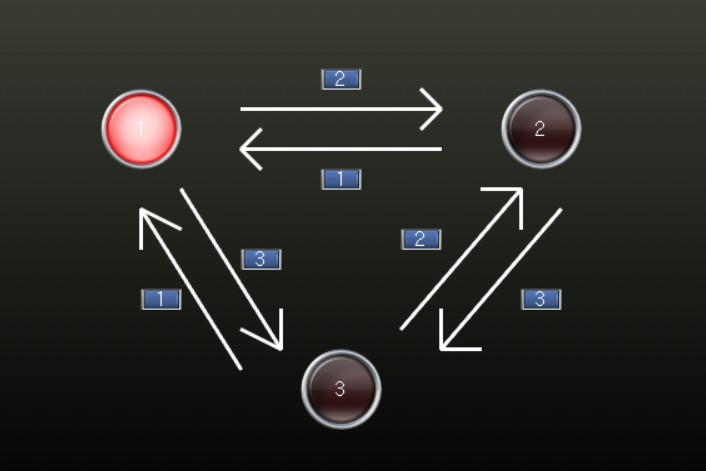
\includegraphics[width=160mm]{../images/laby/grafstanow_tras.jpg}
    \caption{Wygląd grafu stanów dla interfejsu użytkownika}
    %\label{fig:normal}
    \end{figure}  

%%%%%%%%%%%%%% Podpunkt4
\section{Wizualizacja procesu}

Wizualizacja składa się z wykresów: sygnałów zadanych i zmierzonych (po lewej stronie) oraz wartości sterowania (po prawej stronie). Oba te wykresy są odpowiednio podpisane. Dodatkowo na dole ekranu wypisywane są wartości aktualne. W prawym dolnym rogu można zauważyć dwie diody, które informują o zmianie kierunku ruchu silnika.

 \begin{figure}[h]
    \centering
    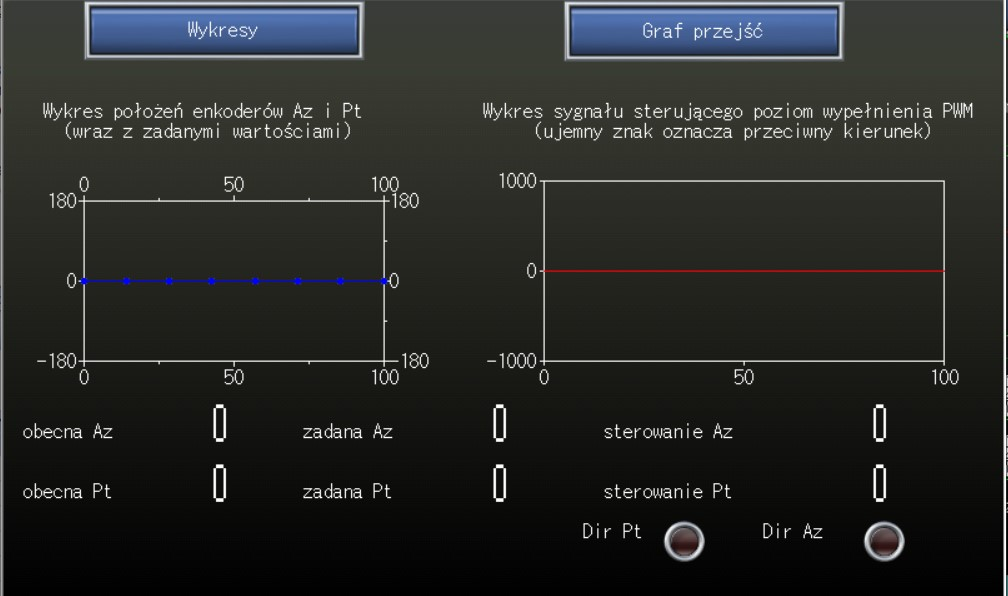
\includegraphics[width=160mm]{../images/laby/wizualizacja_tras.jpg}
    \caption{Wygląd interfejsu użytkownika (wizualizacja)}
    %\label{fig:normal}
    \end{figure}  
